\documentclass{article}

\usepackage{graphicx}
\usepackage{tikz}
\usepackage{tikzsymbols}
\usetikzlibrary{calc,patterns,shapes.geometric}
\pagestyle{empty}
\usepackage[margin=0pt]{geometry}
\geometry{papersize={14in,12in}}

\def\centerarc[#1](#2)(#3:#4:#5){\draw[#1] ($(#2)+({#5*cos(#3)},{#5*sin(#3)})$) arc (#3:#4:#5);}

\begin{document}
	\begin{figure}
		\centering
		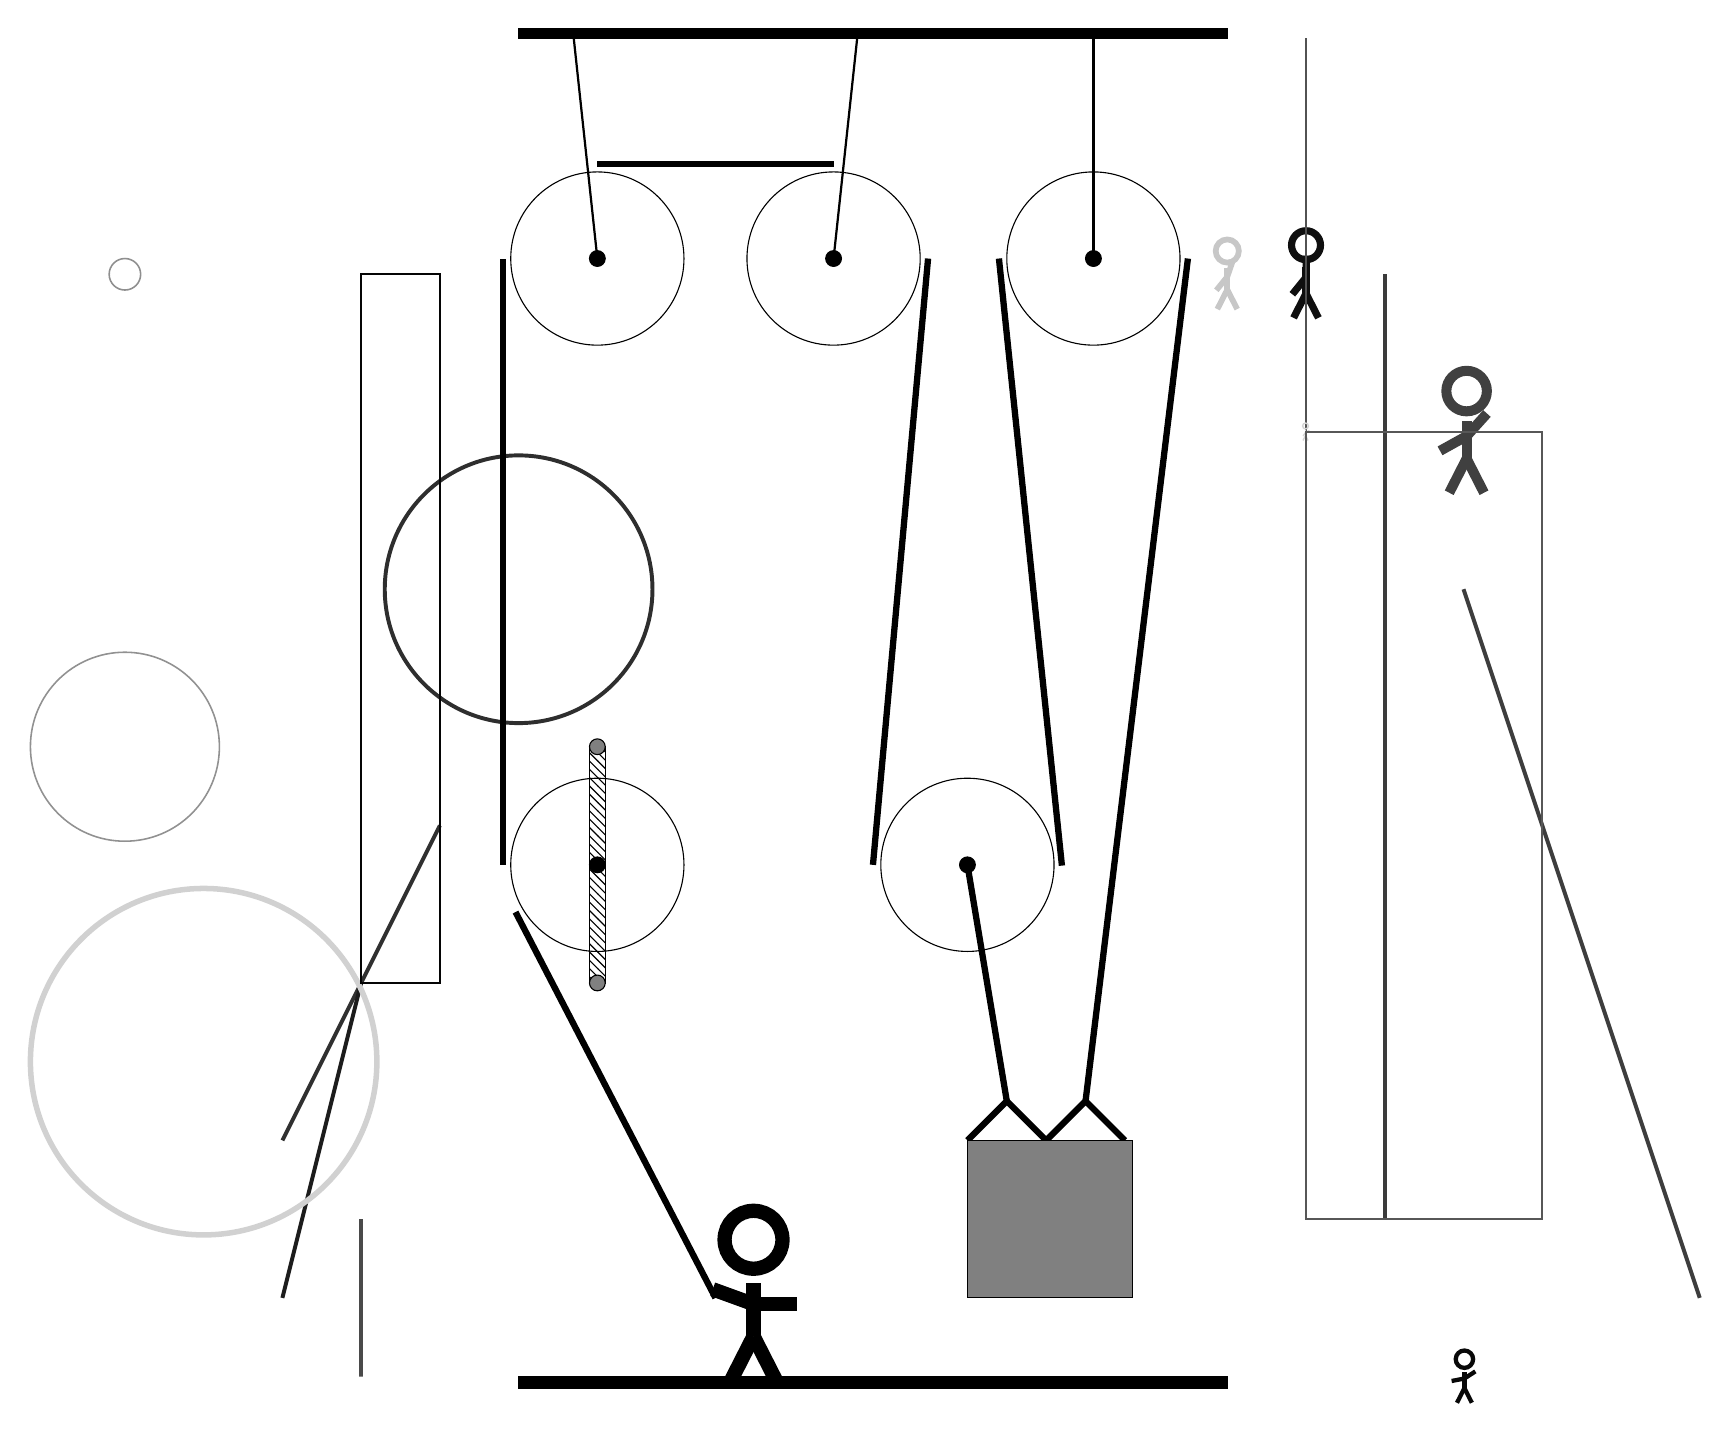
\begin{tikzpicture}
			%%%%% START %%%%%
			
			\draw[fill=black] (-3, 14) rectangle (6, 14.125);
			
			\draw (1, 11.2) circle (1.1);
			\draw[fill=black] (1, 11.2) circle (0.1);
			\draw[thick] (1, 11.2) -- (1.3, 14);
			
			\draw (4.3, 11.2) circle (1.1);
			\draw[fill=black] (4.3, 11.2) circle (0.1);
			\draw[thick] (4.3, 11.2) -- (4.3, 14);
			
			\draw (2.7, 3.5) circle (1.1);
			\draw[fill=black] (2.7, 3.5) circle (0.1);
			
			\draw[line width=0.8mm]  (2.7, 0) -- (3.2, 0.5) -- (3.7, 0) -- (4.2, 0.5) -- (4.7, 0);
			\draw[fill=black!50] (2.7, 0) rectangle (4.8, -2);
			
			\draw (-2, 11.2) circle (1.1);
			\draw[fill=black] (-2, 11.2) circle (0.1);
			\draw[thick] (-2, 11.2) -- (-2.3, 14);
			
			\node[line width=0.5mm, color=black!22] at (6, 11) {\Strichmaxerl[4][51][71]};
			
			\draw [line width=0.5mm, color=black!82](-3, 7) circle (1.7);
			\node[line width=0.7mm, color=black!75] at (9, 9) {\Strichmaxerl[7][29][48]};
			\node[line width=0.4mm, color=black!97] at (9, -3) {\Strichmaxerl[3][11][33]};
			
			\draw [line width=0.2mm, color=black!43](-8, 5) circle (1.2);
			
			\draw[line width=0.5mm, color=black!71] (-5, -1) rectangle (-5, -3);
			\node[line width=0.4mm, color=black!94] at (7, 11) {\Strichmaxerl[5][51][89]};
			\draw[line width=0.5mm, color=black!81](-6, 0) -- (-4, 4);
			\draw[line width=0.2mm, color=black!68] (7, -1) rectangle (7, 14);
			
			\draw [line width=0.2mm, color=black!44](-8, 11) circle (0.2);
			\draw[line width=0.5mm, color=black!89](-5, 2) -- (-6, -2);
			\draw[line width=0.5mm, color=black!77](8, 11) -- (8, -1);
			\draw [line width=0.7mm, color=black!18](-7, 1) circle (2.2);
			
			\node[line width=0.6mm, color=black!17] at (7, 9) {\Strichmaxerl[1][57][26]};
			\draw[line width=0.5mm, color=black!76](9, 7) -- (12, -2);
			\draw[line width=0.3mm, color=black!98] (-5, 11) rectangle (-4, 2);
			
			\draw[line width=0.2mm, color=black!66] (7, 9) rectangle (10, -1);
			
			
			\draw (-2, 3.5) circle (1.1);
			\draw[fill=black] (-2, 3.5) circle (0.1);
			\draw[pattern=north west lines, pattern color=black] (-2.1, 5.0) rectangle (-1.9, 2.0);
			\draw[fill=black!50] (-2, 5.0) circle (0.1);
			\draw[fill=black!50] (-2, 2.0) circle (0.1);
			
			\draw[line width=0.8mm](-0.5, -2) -- (-3.0392, 2.9);
			\centerarc[line width=0.8mm](-2, 3.5)(180:210:1.2000000000000002);
			\draw[line width=0.8mm](-3.2, 3.5) -- (-3.2, 11.2);
			\centerarc[line width=0.8mm](-2, 11.2)(90:180:1.2000000000000002);
			
			\draw[line width=0.8mm](-2, 12.4) -- (1, 12.4);
			\centerarc[line width=0.8mm](1, 11.2)(0:90:1.2000000000000002);
			\draw[line width=0.8mm](2.2, 11.2) -- (1.5, 3.5);
			\centerarc[line width=0.8mm](2.7, 3.5)(180:370:1.2000000000000002);
			\draw[line width=0.8mm] (3.9, 3.49) -- (3.1, 11.2);
			\centerarc[line width=0.8mm](4.3, 11.2)(0:180:1.2000000000000002);
			\draw[line width=0.8mm](4.2, 0.5) -- (5.5, 11.2);
			\draw[line width=0.8mm] (3.2, 0.5) -- (2.7, 3.5);
			
			\node at (0, -2) {\Strichmaxerl[10][-20][0]};
			
			\draw[fill=black] (-3, -3) rectangle (6, -3.15);
			
			%%%%% END %%%%%
		\end{tikzpicture}
	\end{figure}	
\end{document}